%\documentclass[openright,twoside,headsepline]{scrbook}
%\usepackage[applemac]{inputenc}
%\usepackage{graphicx,xcolor,hyperref} % obsolete in HU-diss
%\usepackage[round,authoryear]{natbib}
%\setlength\bibhang{2em} 
%
%
%\KOMAoptions{numbers=noenddot}
\usepackage{amsmath,amssymb,amsfonts,amsthm,epigraph,scrpage2}
\usepackage[ngerman,english]{babel}
\definecolor{Cayenne}{rgb}{0.502,0.0,0.0}
\definecolor{Steel}{rgb}{0.4,0.4,0.4}


%\setcounter{secnumdepth}{3} % sub subsections numbering
%\setcounter{tocdepth}{3} % subsubsections inTOC

\usepackage[format=plain,singlelinecheck=false, font={sf,small},labelfont={bf,color=Steel}]{caption}
\DeclareCaptionLabelSeparator{cayenne_period}{\textcolor{Cayenne}{.} }
\captionsetup{labelsep=cayenne_period}

% Colors
\addtokomafont{chapter}{\color{Steel}}
\addtokomafont{section}{\color{Steel}}
\addtokomafont{subsection}{\color{Steel}}
\addtokomafont{subsubsection}{\color{Steel}}
\addtokomafont{paragraph}{\color{Steel}}

\addtokomafont{pagehead}{\color{Steel}}
\renewcommand{\pnumfont}{\color{Steel}} 
\addtokomafont{headsepline}{\color{Steel}} 
\pagestyle{scrheadings} 

%\makeatletter % dot after sections and all below
%\let\std@sect\@sect
%\def\@sect#1#2#3#4#5#6[#7]#8{\std@sect{#1}{#2}{#3}{#4}{#5}{#6}[#7.]{#8\color{Cayenne}{.}}}
%\makeatother

\usepackage[leftcaption]{sidecap} % inner, outer,left,right
\sidecaptionvpos{figure}{t}

% Papiergr��e
%\setlength{\paperwidth}{24cm}
%\setlength{\paperheight}{17cm}
%\recalctypearea
%\usepackage{geometry}

%% Flattersatz
%\usepackage[document]{ragged2e} % Flattersatz
%\setlength{\RaggedRightParindent}{1em} % evtl. parskip


%% Sans Serif
%\usepackage{cmbright}
%\renewcommand{\familydefault}{\sfdefault}
%% Palatino
%\usepackage[sc]{mathpazo}
%\linespread{1.05}         % Palatino needs more leading (space between lines)
%\setkomafont{sectioning}{\normalcolor\bfseries} % Kapitel�berschriften

%%% Kapitel�berschriften: Mit gro�en Zahlen
%\usepackage{titlesec}
%\titleformat{\chapter}[display]
%{\bfseries\Large}
%{ %\Huge\textsc{\chaptertitlename} % f�r das Wort 'Kapitel'
%\hfill\fontsize{120}{70}\selectfont\color{lightgray}\textbf{\thechapter}}
%{-2ex}
%%{\filleft\fontsize{50}{70}\selectfont\scshape} % Kapit�lchen oder...
%{\filleft\fontsize{50}{70}\selectfont\textbf} % ...oder keine Kapit�lchen
%[\vspace{0ex}]
%
%%%% Part�berschriften
%\titleformat{\part}[display]
%{\bfseries\Large}
%{ %\Huge\textsc{\chaptertitlename} % f�r das Wort 'Kapitel'
%\hfill\fontsize{120}{70}\selectfont\color{lightgray}\textbf{\thepart}}
%{-2ex}
%{\filleft\fontsize{50}{70}\selectfont\scshape} % Kapit�lchen oder...
%%{\filleft\fontsize{50}{70}\selectfont\textbf} % ...oder keine Kapit�lchen
%[\vspace{0ex}]


\newcommand{\ER}{Erd\H{o}s-R\'enyi }
\newcommand{\BA}{Barab\'asi-Albert }
\newcommand{\mean}[1]{\left< #1 \right>}
\newcommand{\abs}[1]{\left| #1 \right|}
\newcommand{\norm}[1]{\lVert#1\rVert}
\newcommand{\mat}[1]{\mathbf{#1}}
\newcommand{\tgraph}{\mathcal{G}}

\theoremstyle{definition} % non-italic
\newtheorem{annahme}{Annahme} % braucht amsthm
\newtheorem{definition}{Definition}
\newtheorem{theorem}{Theorem}
\newtheorem{satz}{Satz}
\newtheorem{frage}{Frage}
%\input{watermarks/watermark.tex}
\DeclareMathOperator{\nnz}{nnz}

% + Graphicspath nach begin document

%
%
%
%\begin{document}
%\graphicspath{{/Users/lentz/Documents/GitHub_locals/Thesis/images/}}
%\tableofcontents
%


\chapter{Static livestock trade network}
In this chapter, we address the analysis of static networks, where the focus lies on epidemic spread on networks.
Large amounts of data about different contact structures between a huge amount of subjects became available in the last years.
In the context of epidemics, different types of networks can be obtained.
Concerning infectious diseases of humans, it is unlikely to have the exact contact data of a (sub)-population.
Different methods to extract the contacts structure can be used \citep{Keeling:2005}:
\emph{Contact tracing} is used to determine infection paths under the assumption that every contact has a high probability to cause an infection.
This assumption is justified for highly contagious diseases, such as influenza or sexually transmitted diseases \citep{Rocha_pnas,Rocha_plosbc}.
If more data is available, one can obtain an \emph{infection tracing} network, where every contact definitely caused an infection.
Infection tracing plays an important role for the analysis of HIV spread or food safety \citep{Wilking,Haydon22012003}.
\emph{Diary-based} methods make use of questionnaires to extract contact structures.
The drawback of this method is that the subjects themselves are responsible for the information given and a considerable bias can be present in the data \citep{Visser:2003p784}.
Other diary-based methods make use of legislation in order to guarantee for a sufficient data quality.
An example is the HI-Tier database, which records trade movements of livestock animals and is used for food safety and is a central subject of study in this work \citep{Euro-Lex}.

Based on the amount of available data as quoted above, it is reasonable to model epidemics using a purely topological analysis.
Detailed epidemiology is by far more complex as solving differential equations.
Fine-grained models including large sets of parameters and couplings are needed to model infectious diseases.
A complex example for the transmission of classical swine fever is found in \citep{MartinezLopez:2011db}.
In general, a detailed knowledge about infection probability, contact probability and sensitivity to initial conditions is required to obtain a realistic epidemic model.
Even if this information was available, results could not necessarily be generalized to other systems.

For this reason we restrict the epidemiological aspect of this work to a purely topological analysis of the underlying networks, where detailed data about contact structures is available.
In particular, we focus on a network of pig trade in Germany in the years 2009--2010.
Each node in this network represents an agricultural holding and trade contacts between holdings are represented by directed edges.
(An analogue analysis of a cattle network dataset was published in \citep{Lentz2009}).
This chapter is devoted to a static network analysis of this system and a general topological classification.
In section XX we highlight the effects of a time-resolved treatment of these systems.

\paragraph{Livestock trade dataset\color{Cayenne}{.}}
After the BSE crisis in Europe in 2001, the EU member states established livestock trade movement databases to track potential pathways of pathogen spread.
Since 2001, every holding in Germany is obliged to report every trade movement of live animals (pig, cattle, sheep and goat) to a federal database (\foreignlanguage{ngerman}{Herkunftssicherungs und Informationssystem f�r Tiere} (HIT), \citep{HI-Tier}).
We focus on the trade contacts for pigs.
Trade is recorded in a temporal resolution of 1 day, where the receiving holding and the pre-owner are reported in the database.
In this section we aggregate the trade contacts yielding a static network, where a trade edge is present, if there was at least one trading contact during the observation period.
Our data extract spans the trade within Germany between january 2009 and march 2010.
This yields a static network with 89,745 nodes and 210,696 edges.


\section{Network analysis}\label{sec:network_analysis}
To begin with, we analyze the livestock trade data according to the measures introduced in section \ref{sec:network_measures}.
\paragraph{Centrality and distances\color{Cayenne}{.}}
Figure \ref{fig:hit_deg_cdf} shows the heavy-tailed degree distribution of the network.
%
\begin{SCfigure}
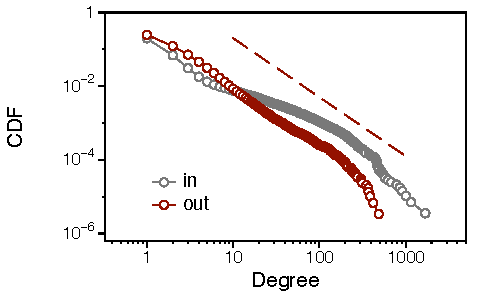
\includegraphics{HIT_Degree_CDF.pdf}
\caption{Degree distribution of the livestock trade network. The out-degree distribution (red) is well approximated by a power-law of the form $x^{-1.6}$ (red dashed line).
The in-degree distribution shows a bimodal behavior indicating large slaughterhouses.
}
\label{fig:hit_deg_cdf}
\end{SCfigure}
%

\paragraph{Components and ranges\color{Cayenne}{.}}
Ignoring the edge direction, the network has a giant component containing more than 98~\% of the nodes. The second largest weakly connected component contains only 11 nodes.
The size of the largest and second largest strongly connected components are 21,8~\% and  0.05~\% (47 nodes), respectively.
Sizes of the next smaller components decrease rapidly.
All in all the network percolates ignoring the direction of links.
Taking into account link directions, the giant component contains a considerable fraction of the network, but is far from the percolation threshold.

The giant strongly connected component has an interesting impact on the distribution of node ranges (and reachabilities) in the network.
Note that the range of a node defines the upper bound for any disease outbreak starting from this very node.
Following equation \eqref{eq:range_def}, we compute the ranges of all nodes and focus for the moment on the \emph{sequence} of these ranges. 
For most sequences of centralities in a network, we would find rather noisy signals.
These signals result in distributions such as the degree distribution in figure \ref{fig:hit_deg_cdf}.
In contrast to most other centrality measures, the range shows a strikingly different behavior.
The sequence of ranges for all nodes in the network is shown in figure \ref{fig:node_range}. 
%
\begin{figure}[htbp]
\begin{center}
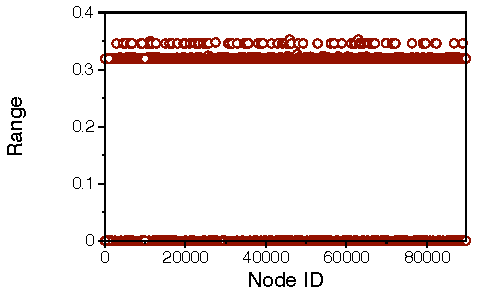
\includegraphics{Node_Range.pdf}
\caption{Range sequence for all nodes in the livestock trade network.
The sequence shows a clear gap in the possible range values and a smaller second gap for the top ranged nodes.
Nodes with range smaller than 10 are not shown.
}
\label{fig:node_range}
\end{center}
\end{figure}
%
The striking feature here is the \emph{gap} in the distribution: no range in between $7\cdot 10^{-4}$ (66 nodes) and $0.32$ (28630 nodes) is present in the system.
There is another, smaller gap for values between $0.33$ (29325 nodes) and $0.35$ (31033 nodes).
Consequently, a randomly chosen node can only belong to one of two classes, namely long ranged nodes and short ranged nodes.
A node of the latter class is barely suitable to cause a considerable disease outbreak at all.
Only a node of long range can act as a node for large scale disease outbreaks.
The sizes of the classes in figure \ref{fig:node_range} are as follows: 41792 nodes belong to the short range and 47953 nodes to the long range class, respectively.
91 nodes of the latter are above the second range gap.

For a general network we define the range gap $\Gamma $ as the size of the largest interval, where the range distribution is identically zero \citep{Lentz:2012pre}.
The balance of the distribution around the gap is measured in terms of the variable
\[
b=\frac{N_\mathrm{l}-N_\mathrm{s}}{N},
\]
where $N$ is the number of nodes and $N_\mathrm{l}$ and $N_\mathrm{s}$ are the numbers of long and short ranged nodes, respectively.
Apparently $b=1$, if all nodes are long ranged and $b=-1$ for only short ranged nodes in the network.
Figure \ref{fig:ER_range_gaps} shows the range gap and balance for directed \ER networks of varying density.
The figure demonstrates, that the size of the range gap and the balance are inherently related to the percolation properties of the system (see section \ref{sec:er_model}).
A significant range gap in combination with equally sized range classes indicates that the system is in a critical state.
For the dataset of figure \ref{fig:node_range} we get $\Gamma = 0.318$ and $b=0.069$ indicating that the system is only slightly above the critical point.
%
\begin{SCfigure}
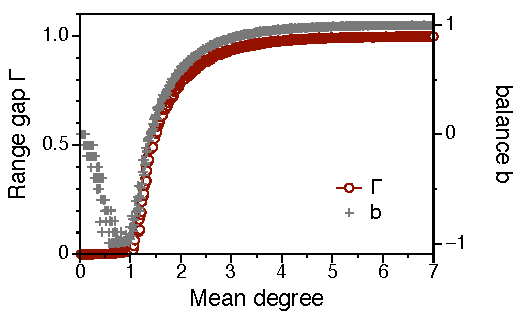
\includegraphics{ER_Range_gap.pdf}
\caption{Range gap $\Gamma $ and balance $b$ vs. mean degree for directed \ER graphs.
Each datapoint is a mean value of 1000 networks. Network size: 1000 nodes.
}
\label{fig:ER_range_gaps}
\end{SCfigure}


The explanation for the strong bi-modality of the range distribution is the existence of a giant strongly connected component (GSCC).
Figure \ref{fig:rangegap_principle} shows a schematic picture of a directed network.
Due to the giant component in the system, all nodes that belong to the GSCC can reach all other nodes in the component plus all nodes that the component is connected to.
%
\begin{figure}[htbp]
\begin{center}
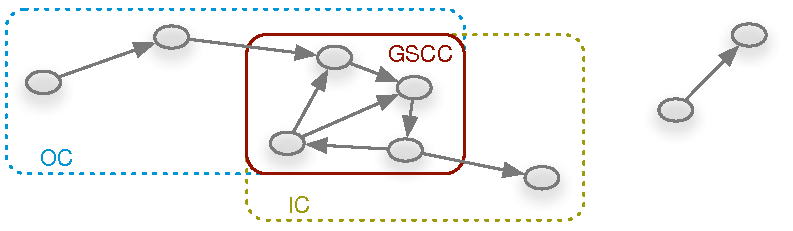
\includegraphics{RangeGap-principle.pdf}
\caption{Schematic structure of a directed network.
In the core region there is the giant strongly connected component (GSCC, red). All nodes reachable from the GSCC form the giant out-component (GOC, yellow) and the nodes with access to the GSCC define the giant in-component (GIC, blue).
The union of GSCC, GIC, GOC and all tendrils is the giant weakly connected component (GWCC) of the network.
Nodes that are not part of the GWCC belong to another component of the network (nodes on the upper right).
}
\label{fig:rangegap_principle}
\end{center}
\end{figure}
%
If there is a path from a node to the GSCC, but the node itself is not on this component, it belongs to the giant in-component (GIC) of the network. 
In analogy, nodes reachable from the GSCC that are themselves not part of the latter, belong to the giant out-component (GOC).
All remaining nodes not belonging to one of the components mentioned above are called tendrils, if they are weakly connected to the GSCC.
The nodes on the upper right (figure \ref{fig:rangegap_principle}) are not even weakly connected to the GSCC and thus belong to another component of the network.

\paragraph{Modules\color{Cayenne}{.}}
The network components analyzed above make a strict requirement to the connectivity between components.
A weaker requirement would be to allow for the existence of only a few edges between components.
Clusters of this type are called \emph{modules} or \emph{communities}.
The idea of finding modules in networks has been proposed in \citep{Newman06062006}.
In order to detect these structures, a cost function mapping every partition of the network onto a value between 0 and 1 has to be optimized.
\citeauthor{Newman06062006} proposed the modularity $Q$ as an appropriate cost function defined as
\[
Q=\text{(number of edges between communities)}-\text{(expected number of those edges)}
\]
or more formally \citep{Fortunanto2010,Newman06062006}
\begin{equation}\label{eq:modularity}
Q=\frac{1}{2m} \sum _{ij}\left( \mat{A}_{ij}-\frac{k_i k_j}{2m} \right) \delta (c_i,c_j).
\end{equation}
This equation gives the modularity for a network with adjacency matrix $\mat{A}$ and $m$ edges and $k_i$ denotes the degree of the $i$-th node.
The partition of the network is given in the Kronecker delta $\delta (c_i,c_j)$, which is 1, if nodes $i$ and $j$ are in the same community and otherwise 0.
Hence, modularity measures the goodness of a particular partition of the network.
$Q\sim 0$ implies that a given partition of a network does not give a significant modular structure.
Its maximum value is $Q=1$ provided that a network has a strong modular partition \emph{and} the latter is known for the computation of $Q$.
Finding best possible partition that maximizes modularity has been shown to be NP-complete \citep{brandes2007}.
However, several approximate methods -- such as simulated annealing \citep{guimera_mod_SA} and greedy algorithms \citep{Clauset_greedy,Newman:fast_algo} -- to maximize modularity have been proposed.
In order to detect community structure in the pig trade network, we analyze the system using the method of \citeauthor{Newman:fast_algo}.
The results presented in this section are published for a similar dataset in \citep{Lentz:2011}.




%
%\bibliographystyle{apalike}
%\bibliography{/Users/lentz/Documents/GitHub_locals/Thesis/bibliography.bib}
%\end{document}

